\documentclass{article}
\usepackage{tikz}
\usetikzlibrary{shapes.geometric}

\begin{document}

\begin{figure}[h]
    \centering
    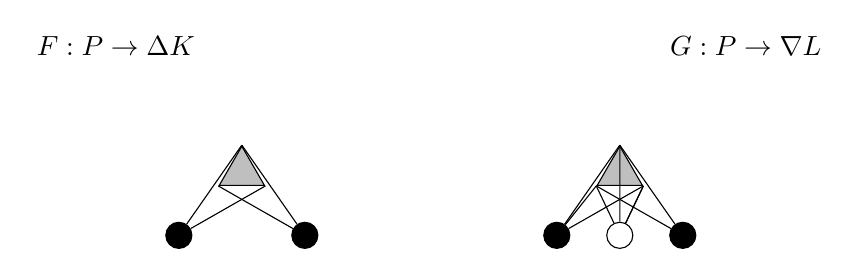
\begin{tikzpicture}[scale=0.8]
        % Define nodes for the left diagram
        \node[draw, fill=gray!50, regular polygon, regular polygon sides=3] (A) at (0,0) {};
        \node[draw, fill=black, circle] (B) at (-1,-1) {};
        \node[draw, fill=black, circle] (C) at (1,-1) {};
        
        % Draw edges for the left diagram
        \draw (A.corner 1) -- (B);
        \draw (A.corner 2) -- (C);
        \draw (A.corner 3) -- (B);
        \draw (A.corner 1) -- (C);
        
        % Define nodes for the right diagram
        \node[draw, fill=gray!50, regular polygon, regular polygon sides=3] (D) at (6,0) {};
        \node[draw, fill=black, circle] (E) at (5,-1) {};
        \node[draw, fill=black, circle] (F) at (7,-1) {};
        \node[draw, fill=white, circle] (G) at (6,-1) {};
        
        % Draw edges for the right diagram
        \draw (D.corner 1) -- (E);
        \draw (D.corner 2) -- (F);
        \draw (D.corner 3) -- (G);
        \draw (D.corner 1) -- (F);
        \draw (D.corner 2) -- (E);
        \draw (D.corner 3) -- (E);
        \draw (D.corner 1) -- (G);
        \draw (D.corner 2) -- (G);
        \draw (D.corner 3) -- (G);
        
        % Labels for the diagrams
        \node at (-2,2) {$F : P \rightarrow \Delta K$};
        \node at (8,2) {$G : P \rightarrow \nabla L$};
    \end{tikzpicture}
\end{figure}

\end{document}